\textbf{CAPOT and typos} When queries have typos, CAPOT is a computationally efficient method of improving performance as the relative gap between unaltered and aligned is greatest on alterations like character deletion, keyboard character replacement, and random character replacement. We attribute this impact to the relative importance of our alignment dataset's character level alterations. Three out of the 10 methods focus on learning alignments based around minor character shifts, and as a result, the performance optimizes there to the detriment of other forms of noise. CAPOT is much less effective in improving the relevance of minor syntactic shifts such as lemmatization or stemming leading to marginal improvements over the unaltered baselines. We attribute this to the already smaller gap on syntactically altered queries, which on datasets such as TriviaQA have less than 2\% impact.\\
\textbf{CAPOT and Retrieval Set Depth} demonstrates that CAPOT, like DA, sees the highest impact when the recall set size is small. On the NQ the gap between CAPOT and the baseline at 20 is nearly 10\% which narrows to ~3\% at 200.  \\
\textbf{Limitations of contrastive alignment} While effective, contrastive alignment has a non-negligible impact on the retrieval accuracy of unaltered queries. As shown in table \ref{tab:capot-nq-20} on non-noisy queries the use of data augmentation incurs no loss in accuracy yet CAPOT incurs ~2.5\%. This is a fundamental issue because the alignment of embeddings causes minor variations in representations that have actual implications on retrieval accuracy. We believe that the use of larger datasets could such as the web search logs used by the Generic Intent Representation of query vectors \cite{Zhang2019GenericIR} could improve this.\\
\textbf{Poly Encoding} using alignment-based optimization we believe leads to novel retrieval methods which allow for fixed index, constrained optimizations tailored to specific types of noise or deficiencies in retrieval. Novel forms of noise-optimized encoders can be deployed in parallel without additional index generation. Given the prevalence of bi-encoders as candidate set generation tools, CAPOT, unlike Data Augmentation, can generate many targeted query encoder variants which share a document representation. As shown in figure \ref{fig:fig2}, instead of seeking a single query encoder that learns all surface and semantic forms of query representations, alignment approaches can be used to create many encoders which are tuned to various goals. 
\label{app:poly-encoder}
\begin{figure}[htb!]
    \centering
    \scalebox{0.22}{
    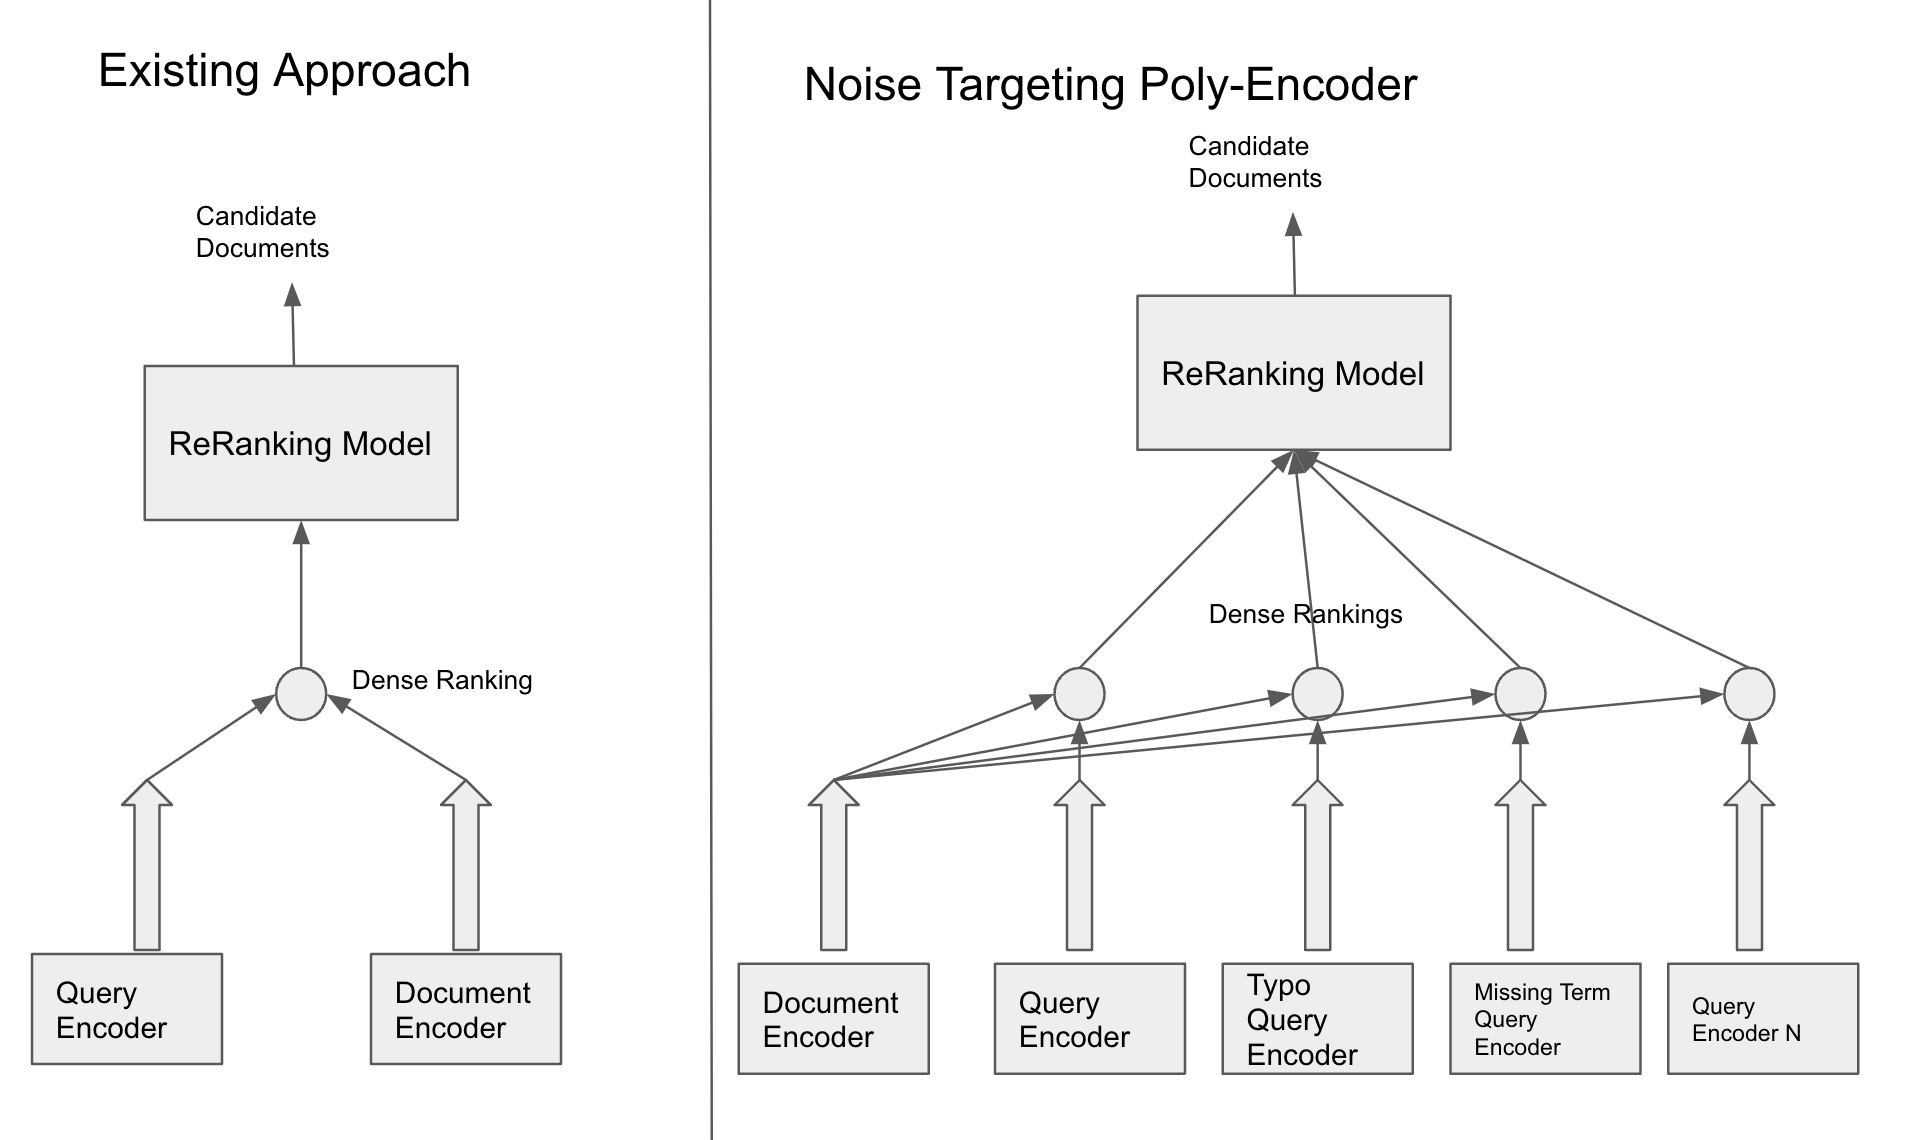
\includegraphics{figure2.png}}
    \caption{Proposed poly-encoder architecture using noise-targeted query encoders optimized with CAPOT}
    \label{fig:fig2}
\end{figure}